\documentclass[10pt,a4paper]{article}

% =========================================================================
% Packages
% =========================================================================
\usepackage[utf8]{inputenc}
\usepackage[T1]{fontenc}
\usepackage{lmodern}
\usepackage{geometry}
\usepackage{graphicx}
\graphicspath{{Gambar/}}
\usepackage{amsmath,amssymb}
\usepackage{fancyhdr}
\usepackage{titlesec}
\usepackage{booktabs}
\usepackage{tabularx}
\usepackage{array}
\usepackage{caption}
\usepackage{subcaption}
\usepackage{algorithm}
\usepackage{algpseudocode}
\usepackage{hyperref}
\usepackage{microtype}
\usepackage{url}
\usepackage{cite}
\usepackage{float}
\usepackage{placeins}

% =========================================================================
% Page Geometry & Margins (EPROTIK Standard: A4 Paper, Margins: 2.5 cm all sides)
% =========================================================================
\geometry{
  a4paper,
  top=2.5cm,
  bottom=2.5cm,
  left=2.5cm,
  right=2.5cm,
  headheight=45pt,
  headsep=12pt,
  footskip=22pt
}

% Paragraph settings: Justified, single space
\setlength{\parindent}{0pt}
\setlength{\parskip}{4.5pt}
\linespread{1.0}

% Float Spacing Adjustments
\setlength{\floatsep}{10pt plus 2pt minus 2pt}
\setlength{\textfloatsep}{12pt plus 2pt minus 2pt}
\setlength{\intextsep}{10pt plus 2pt minus 2pt}

% Hyperlink configuration
\hypersetup{
  colorlinks=true,
  linkcolor=blue,
  citecolor=blue,
  urlcolor=blue
}

% =========================================================================
% Header & Footer Settings
% =========================================================================
\pagestyle{fancy}
\fancyhf{}
\fancyhead[L]{\fontsize{9pt}{11pt}\selectfont eProceeding of TIK}
\fancyfoot[R]{\fontsize{9pt}{11pt}\selectfont\thepage}
\renewcommand{\headrulewidth}{0.4pt}
\renewcommand{\footrulewidth}{0pt}

% First page header
\fancypagestyle{firstpage}{
  \fancyhf{}
  \fancyhead[L]{%
    \begin{minipage}[c]{0.78\textwidth}
      {\fontsize{10pt}{12pt}\selectfont\textbf{eProceeding of TIK}}\\[2pt]
      {\fontsize{8.5pt}{10.5pt}\selectfont E-ISSN: 2797-1724, P-ISSN: 3031-1454}\\[1pt]
      {\fontsize{8.5pt}{10.5pt}\selectfont Vol. 7 No. 1 2027 pp. xx--xx}
    \end{minipage}%
  }
  \fancyhead[R]{%
    \begin{minipage}[c]{0.20\textwidth}
      \raggedleft
      \IfFileExists{Gambar/template_eprotik_image5.png}{
\includegraphics[height=1.05cm]{template_eprotik_image5.png}}{%
        \IfFileExists{Gambar/elvira_image5.png}{
\includegraphics[height=1.05cm]{elvira_image5.png}}{}%
      }
    \end{minipage}%
  }
  \fancyfoot[R]{\fontsize{9pt}{11pt}\selectfont\thepage}
  \renewcommand{\headrulewidth}{0.5pt}
  \renewcommand{\footrulewidth}{0pt}
}

% =========================================================================
% Section Headings Formatting
% Level 1: 14pt Bold
% Level 2: 12pt Bold
% Level 3: 10pt Bold
% =========================================================================
\titleformat{\section}
  {\fontsize{14pt}{17pt}\bfseries}{\thesection.}{0.5em}{}
\titlespacing*{\section}{0pt}{12pt}{4pt}

\titleformat{\subsection}
  {\fontsize{12pt}{15pt}\bfseries}{\thesubsection}{0.5em}{}
\titlespacing*{\subsection}{0pt}{9pt}{3pt}

\titleformat{\subsubsection}
  {\fontsize{10pt}{12pt}\bfseries}{\thesubsubsection}{0.5em}{}
\titlespacing*{\subsubsection}{0pt}{6pt}{2pt}

% Caption styles (9 pt / small)
\captionsetup{font={small},labelfont=bf,justification=centering}
\captionsetup[table]{position=top,skip=3pt}
\captionsetup[figure]{position=bottom,skip=4pt}

% =========================================================================
% Document Body
% =========================================================================
\begin{document}
\thispagestyle{firstpage}

% --- Article Title (22pt Bold, Left Aligned) ---
{\fontsize{20pt}{25pt}\bfseries\raggedright Panduan Penulis untuk Jurnal Teknologi Rekayasa Informasi dan Komputer (Rata Kiri, Tebal, Ukuran Huruf 22 Pt)\par}
\vspace{8pt}

% --- Authors (11pt Regular) ---
{\fontsize{11pt}{13pt}\selectfont Nama Penulis Pertama$^{1}$, Nama Penulis Kedua$^{2*}$, Nama Penulis Ketiga$^{3}$, Nama Penulis Keempat$^{4}$ (11 pt)\par}
\vspace{4pt}

% --- Affiliations (9pt) ---
{\fontsize{9pt}{11pt}\selectfont
$^{1,2}$ Nama Departemen atau Fakultas, Nama Universitas atau Organisasi, Negara (9 pt)\par
$^{3}$ Nama Departemen atau Fakultas, Nama Universitas atau Organisasi, Negara\par
$^{4}$ Nama Departemen atau Fakultas, Nama Universitas atau Organisasi, Negara\par}
\vspace{4pt}

% --- Corresponding Author (9pt) ---
{\fontsize{9pt}{11pt}\selectfont
*Penulis Korespondensi: \href{mailto:penuliskedua@uni.edu.tw}{penuliskedua@uni.edu.tw} (9 pt)\par}
\vspace{4pt}

% --- Open Access License (8pt) ---
{\fontsize{8pt}{10pt}\selectfont
This is an open access article under the \href{https://creativecommons.org/licenses/by-sa/4.0/}{CC BY-SA} license. 
\IfFileExists{Gambar/template_eprotik_image1.png}{\raisebox{-0.10cm}{
\includegraphics[height=0.40cm]{template_eprotik_image1.png}}}{%
  \IfFileExists{Gambar/elvira_image1.png}{\raisebox{-0.10cm}{
\includegraphics[height=0.40cm]{elvira_image1.png}}}{}%
}\par}

\vspace{5pt}
\noindent\rule{\textwidth}{0.4pt}
\vspace{3pt}

% --- Abstrak (14pt Heading, 10pt Content) ---
{\fontsize{14pt}{16pt}\bfseries Abstrak (14 pt)\par}
\vspace{4pt}

{\fontsize{10pt}{13pt}\selectfont
Abstrak biasanya disajikan secara terpisah dari artikel, sehingga harus dapat berdiri sendiri. Abstrak yang disusun dengan baik memungkinkan pembaca untuk mengidentifikasi isi dasar dari suatu dokumen dengan cepat dan akurat, menentukan relevansinya dengan minat mereka, dan memutuskan apakah akan membaca dokumen tersebut secara keseluruhan. Abstrak harus bersifat informatif dan sepenuhnya dapat menjelaskan isi artikel, memberikan pernyataan yang jelas mengenai permasalahan, pendekatan atau solusi yang diusulkan, serta menyoroti temuan dan kesimpulan utama. Panjang abstrak harus antara 100 hingga 200 kata. Referensi sebaiknya dihindari, namun jika sangat penting, cantumkan nama penulis dan tahun. Gunakan nomenklatur standar, dan hindari singkatan yang tidak umum atau tidak standar. Namun, jika harus digunakan, maka harus didefinisikan pada penyebutan pertama dalam abstrak. Tidak diperbolehkan mengutip literatur. Daftar kata kunci memberikan kesempatan untuk mencantumkan 5 hingga 7 kata kunci, yang akan digunakan oleh layanan pengindeksan dan abstraksi, selain yang sudah terdapat dalam judul. (10 pt)\par}

\vspace{5pt}
{\fontsize{10pt}{12pt}\selectfont\textbf{Kata kunci:} satu, dua, tiga, empat, lima\par}

\vspace{4pt}
\noindent\rule{\textwidth}{0.4pt}
\vspace{6pt}

% =========================================================================
% Section 1: Pendahuluan (14pt)
% =========================================================================
\section{Pendahuluan (14 pt)}

Format teks utama terdiri dari kolom kiri-kanan rata pada kertas ukuran A4 (kuarto). Margin teks dari kiri, kanan, bawah, dan atas adalah 2,5 cm. Naskah ditulis menggunakan Microsoft Word, spasi tunggal, huruf Twentieth Century ukuran 10 pt, dengan maksimal 12 halaman untuk artikel penelitian asli, atau maksimal 16 halaman untuk artikel tinjauan/review, yang dapat diunduh melalui situs web: \url{https://e-jurnal.pnl.ac.id/eProTIK}.

Judul artikel harus terdiri dari kata-kata seminimal mungkin yang secara akurat menggambarkan isi makalah. Judul harus ringkas dan informatif, tidak lebih dari sekitar 12 kata. Jangan gunakan akronim atau singkatan dalam judul, dan jangan mencantumkan metode yang digunakan, kecuali jika makalah tersebut membahas pengembangan metode baru. Judul sering digunakan dalam sistem pencarian informasi. Hindari menulis rumus panjang dengan subskrip dalam judul. Hilangkan kata-kata yang tidak perlu seperti ``Studi tentang...'', ``Penelitian terhadap...'', ``Implementasi dari...'', ``Pengamatan terhadap...'', ``Pengaruh...'', ``Analisis...'', ``Perancangan...'', dan sejenisnya.

Abstrak yang ringkas dan faktual diperlukan. Abstrak harus menyatakan secara singkat tujuan penelitian, hasil utama, dan kesimpulan penting. Abstrak biasanya disajikan secara terpisah dari artikel, sehingga harus dapat berdiri sendiri. Karena alasan ini, referensi sebaiknya dihindari, namun jika sangat penting, maka cantumkan nama penulis dan tahun. Singkatan yang tidak umum sebaiknya dihindari, namun jika diperlukan harus dijelaskan pada penyebutan pertama dalam abstrak. Segera setelah abstrak, berikan maksimal 7 kata kunci, menggunakan ejaan Amerika dan hindari istilah umum, bentuk jamak, dan konsep majemuk (misalnya hindari penggunaan kata ``dan'', ``dari''). Gunakan singkatan secara hemat: hanya singkatan yang sudah umum digunakan di bidang tersebut yang boleh digunakan. Kata kunci ini akan digunakan untuk keperluan pengindeksan.

Layanan pengindeksan dan abstraksi sangat bergantung pada keakuratan judul, karena judul akan digunakan untuk mengambil kata kunci yang bermanfaat dalam pencocokan silang dan pencarian komputer. Judul yang tidak tepat dapat menyebabkan artikel tidak pernah menjangkau audiens yang dituju, oleh karena itu judul harus spesifik.

Bagian pendahuluan harus memuat: i) latar belakang yang jelas, ii) pernyataan masalah yang jelas, iii) tinjauan pustaka yang relevan, iv) pendekatan atau solusi yang diusulkan, dan v) nilai kebaruan dari penelitian, yaitu inovasi (ditulis dalam 3--6 paragraf). Pendahuluan harus dapat dipahami oleh rekan sejawat dari berbagai disiplin ilmu. Penulisan dan sitasi pustaka menggunakan gaya IEEE dengan tanda \cite{sigala2019big}, \cite{nguyen2019machine}, dan seterusnya. Istilah dalam bahasa asing ditulis dalam huruf \textit{italic}. Teks harus dibagi ke dalam beberapa bagian, masing-masing dengan judul tersendiri dan diberi nomor secara berurutan, misalnya: 1. PENDAHULUAN. Biasanya, artikel lengkap berisi: 1. PENDAHULUAN, 2. DASAR TEORI DAN/ATAU METODE/ALGORITMA YANG DIAJUKAN (opsional), 3. METODE, 4. HASIL DAN PEMBAHASAN, and 5. KESIMPULAN. Struktur ini dikenal sebagai gaya IMRaD.

Tinjauan pustaka yang dilakukan penulis digunakan dalam bagian PENDAHULUAN untuk menjelaskan perbedaan naskah dengan penelitian sebelumnya (sebagai bentuk inovasi), digunakan dalam bagian METODE untuk menjelaskan tahapan penelitian, dan digunakan dalam HASIL DAN PEMBAHASAN untuk mendukung analisis hasil \cite{nguyen2019machine}. Jika naskah benar-benar memiliki orisinalitas tinggi dan mengusulkan metode atau algoritma baru, maka bagian tambahan setelah PENDAHULUAN dan sebelum METODE dapat ditambahkan untuk menjelaskan secara ringkas teori dan/atau metode atau algoritma yang diusulkan \cite{vinayakumar2019deep}.

% =========================================================================
% Section 2: Metode (14pt)
% =========================================================================
\section{Metode (14 pt)}

Menjelaskan penelitian secara kronologis, termasuk desain penelitian, prosedur penelitian (dalam bentuk algoritma, pseudocode, atau bentuk lainnya), cara pengujian, dan akuisisi data \cite{sivaraman2019network, dwivedi2019decentralized, alturjman2019quantifying}. Uraian mengenai jalannya penelitian harus didukung oleh referensi, agar penjelasan tersebut dapat diterima secara ilmiah \cite{nguyen2019machine, vinayakumar2019deep}. Gambar \ref{fig:contoh_gambar}--\ref{fig:contoh_gabung} dan Tabel \ref{tab:contoh_tabel} disajikan di tengah (\textit{center}), seperti ditunjukkan di bawah ini dan disitasi dalam naskah \cite{sivaraman2019network, kumar2019big, ang2019deployment, lau2019survey, wu2019large, mosavi2019prediction, palanisamy2019implications}. Dampak pelepasan listrik terhadap tingkat keasaman HVNE dan NELV telah diilustrasikan pada Gambar \ref{fig:contoh_gabung}(a), dan dampak tegangan tembus pada NE dan NELV telah diilustrasikan pada Gambar \ref{fig:contoh_gabung}(b).

\begin{figure}[H]
  \centering
  \IfFileExists{Gambar/template_eprotik_image4.jpg}{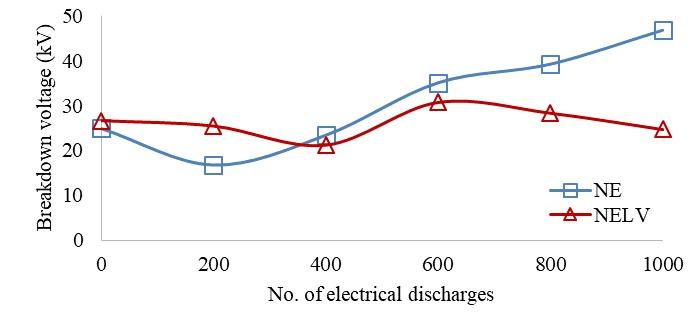
\includegraphics[width=0.60\textwidth]{template_eprotik_image4.jpg}}{\fbox{Contoh Gambar}}
  \caption{Contoh gambar (9 pt)}
  \label{fig:contoh_gambar}
\end{figure}

Contoh tabel ditunjukkan sebagai berikut.

\begin{table}[H]
  \centering
  \caption{Contoh tabel (10 pt)}
  \label{tab:contoh_tabel}
  \fontsize{9pt}{11pt}\selectfont
  \begin{tabular}{ccccc}
    \toprule
    \textbf{Variable (9pt)} & \textbf{Speed (rpm)} & \textbf{Power (kW)} & \textbf{Power (kW)} & \textbf{Power (kW)} \\
    \midrule
    (9 pt) a & 10 & 8.6  & 8.6  & 8.6  \\
    b        & 15 & 12.4 & 12.4 & 12.4 \\
    c        & 20 & 15.3 & 15.3 & 15.3 \\
    d        & 10 & 8.6  & 8.6  & 8.6  \\
    e        & 15 & 12.4 & 12.4 & 12.4 \\
    f        & 20 & 15.3 & 15.3 & 15.3 \\
    \bottomrule
  \end{tabular}
\end{table}

Contoh gambar yang digabung:

\begin{figure}[H]
  \centering
  \begin{subfigure}[b]{0.45\textwidth}
    \centering
    \IfFileExists{Gambar/template_eprotik_image2.png}{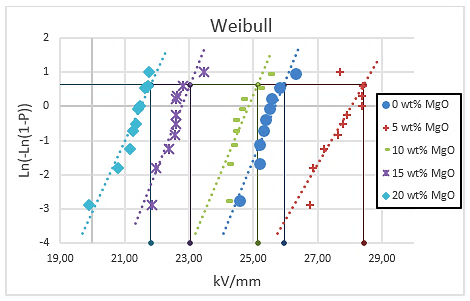
\includegraphics[width=\textwidth]{template_eprotik_image2.png}}{\fbox{Gambar 2(a)}}
    \caption{}
    \label{fig:gabung_a}
  \end{subfigure}
  \hfill
  \begin{subfigure}[b]{0.45\textwidth}
    \centering
    \IfFileExists{Gambar/template_eprotik_image3.png}{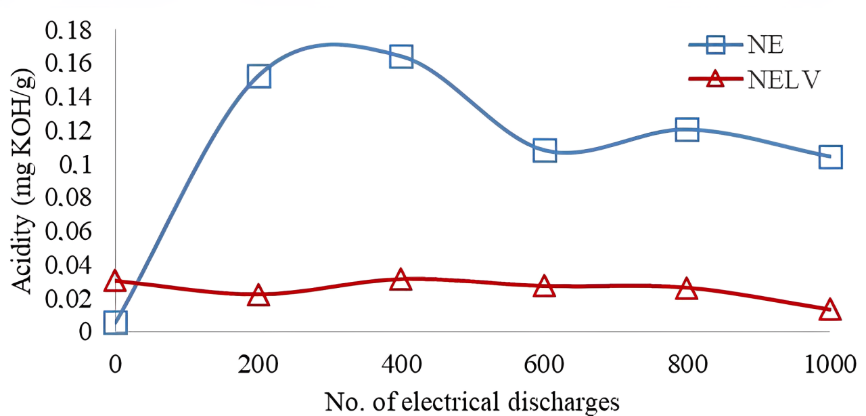
\includegraphics[width=\textwidth]{template_eprotik_image3.png}}{\fbox{Gambar 2(b)}}
    \caption{}
    \label{fig:gabung_b}
  \end{subfigure}
  \caption{Example Effects of electrical discharges to (a) acidity of HVNE and NELV and (b) breakdown voltage of NE and NELV samples (9 pt)}
  \label{fig:contoh_gabung}
\end{figure}

% =========================================================================
% Section 3: Hasil dan Pembahasan (14pt)
% =========================================================================
\section{Hasil dan Pembahasan (14 pt)}

Pada bagian ini dijelaskan hasil penelitian sekaligus disertai dengan pembahasan yang komprehensif. Hasil dapat disajikan dalam bentuk gambar, grafik, tabel, dan bentuk lainnya yang memudahkan pembaca untuk memahami \cite{sadowski2019data, saura2019comparing}. Pembahasan dapat disusun dalam beberapa subbagian.

\subsection{Persamaan (12 pt)}

Persamaan harus diletakkan di tengah baris dan diberi nomor urut dalam tanda kurung yang diratakan ke margin kanan, seperti pada \eqref{eq:contoh_persamaan}. Disarankan untuk menggunakan Microsoft Equation Editor atau MathType.

\begin{equation}
  E_v - E = \frac{\hbar^2}{2m} (k_x^2 + k_y^2)
  \label{eq:contoh_persamaan}
\end{equation}

Semua simbol yang digunakan dalam persamaan harus didefinisikan pada teks setelahnya.

\subsection{Algoritma atau Pseudocode (12 pt)}

Algoritma atau pseudocode ditulis menggunakan font Consolas dengan ukuran 9 pt dan perataan teks kiri. Nama algoritma harus disebutkan dengan jelas. Deskripsi algoritma juga harus dicantumkan sesuai kebutuhan di dalam tabel. Lihat contoh di bawah ini.

\begin{algorithm}[H]
\caption{Greedy search algorithm (10 pt)}
\label{alg:greedy}
\fontsize{9pt}{11pt}\selectfont
\begin{algorithmic}[1]
\Require The algorithm takes as input a graph $G(V,E)$, where $V$ is the set of vertices and $E$ is the set of edges. It also requires a start node $s$, a goal node $g$, and a heuristic function $h(n)$ that estimates the cost from any node $n$ to the goal. The output is a path from the start node $s$ to the goal node $g$, if such a path exists.
\State $\text{Initialize } open\_list \leftarrow [s]$
\State $\text{Initialize } came\_from \leftarrow \text{empty map}$
\While{$open\_list \text{ is not empty}$}
    \State $current \leftarrow \text{node in } open\_list \text{ with lowest } h(current)$
    \If{$current = g$}
        \State \Return $\text{ReconstructPath}(came\_from, current)$
    \EndIf
    \State $\text{remove } current \text{ from } open\_list$
    \For{\textbf{each} $neighbor \text{ in } \text{Neighbors}(current)$}
        \If{$neighbor \text{ not in } came\_from$}
            \State $came\_from[neighbor] \leftarrow current$
            \State $\text{Add } neighbor \text{ to } open\_list$
        \EndIf
    \EndFor
\EndWhile
\State \Return \textbf{failure}
\end{algorithmic}
\end{algorithm}

\subsection{Sitasi (12 pt)}

Sitasi yang tepat terhadap karya orang lain harus dilakukan untuk menghindari plagiarisme. Saat merujuk pada item referensi, gunakan nomor referensi seperti dalam \cite{nallaperuma2019online} atau \cite{schulz2019advanced} untuk beberapa referensi. Penggunaan ``Ref \cite{shang2019data} ...'' digunakan apabila sitasi ditempatkan di awal kalimat. Untuk referensi dengan tiga atau lebih penulis, hanya penulis pertama yang dituliskan diikuti dengan \textit{et al.} (misalnya dalam \cite{yu2019clinical}). Contoh item referensi dari berbagai kategori ditunjukkan pada bagian Daftar Pustaka. Setiap item dalam daftar pustaka harus diketik dengan ukuran font 8 pt \cite{huang2019queuing, xu2019internet, aqib2019smarter, leonelli2020data, stylos2019big, song2017tensor}.

\subsubsection{Subbagian Level 3 (10 pt)}
Lorem Ipsum is simply dummy text of the printing and typesetting industry. Lorem Ipsum has been the industry's standard dummy text ever since the 1500s, when an unknown printer took a galley of type and scrambled it to make a type specimen book.

\subsubsection{Subbagian Level 3 (10 pt)}
Lorem Ipsum is simply dummy text of the printing and typesetting industry. Lorem Ipsum has been the industry's standard dummy text ever since the 1500s, when an unknown printer took a galley of type and scrambled it to make a type specimen book.

% =========================================================================
% Section 4: Kesimpulan (14pt)
% =========================================================================
\section{Kesimpulan (14 pt)}

Berikan pernyataan bahwa apa yang diharapkan sebagaimana dijelaskan dalam bagian ``PENDAHULUAN'' pada akhirnya dapat tercapai dalam bagian ``HASIL DAN PEMBAHASAN'', sehingga terdapat kesesuaian antara tujuan dan hasil penelitian. Selain itu, prospek pengembangan hasil penelitian dan penerapan studi lanjutan juga dapat ditambahkan pada bagian ini, berdasarkan hasil dan pembahasan yang telah diperoleh.

% =========================================================================
% Ucapan Terima Kasih (12pt)
% =========================================================================
\section*{Ucapan Terima Kasih (bila ada) (12 pt)}

Bagian ini harus mencantumkan ucapan terima kasih kepada individu yang memberikan bantuan pribadi terhadap pekerjaan ini namun tidak memenuhi kriteria sebagai penulis, dengan menjelaskan kontribusi mereka secara rinci. Sangat penting untuk memperoleh persetujuan dari semua individu yang dicantumkan dalam bagian ucapan terima kasih.

% =========================================================================
% References (IEEE Style, 12pt heading)
% =========================================================================
\section*{REFERENSI (12 pt)}

\begingroup
\fontsize{10pt}{12pt}\selectfont
Referensi utama harus berasal dari jurnal dan prosiding internasional. Semua referensi harus merujuk pada sumber yang paling relevan dan terkini, dengan jumlah minimum 25 referensi untuk artikel penelitian asli dan 50 referensi untuk artikel tinjauan (\textit{review}). Penulisan referensi mengikuti gaya IEEE. Anda dapat mengakses panduan lengkap di \url{http://ipmuonline.com/guide/refstyle.pdf}.

Gunakan alat manajemen referensi seperti EndNote, Mendeley, atau Zotero untuk membantu dalam pengelolaan dan pemformatan referensi, dan pastikan memilih gaya IEEE. Harap gunakan format yang konsisten dalam penulisan referensi --- lihat contoh berikut (ukuran font 10 pt):

\vspace{4pt}
\textbf{Journal/Periodicals}\\
\textit{Basic Format:}
J. K. Author, ``Title of paper,'' \textit{Abbrev. Title of Journal/Periodical}, vol. x, no. x, pp. xxx--xxx, Abbrev. Month, year, doi: xxx.

\textit{Examples:}
\begin{itemize}
    \setlength{\itemsep}{0pt}
    \setlength{\parskip}{0pt}
    \item M. M. Chiampi and L. L. Zilberti, ``Induction of electric field in human bodies moving near MRI: An efficient BEM computational procedure,'' \textit{IEEE Trans. Biomed. Eng.}, vol. 58, pp. 2787--2793, Oct. 2011, doi: 10.1109/TBME.2011.2158315.
    \item R. Fardel, M. Nagel, F. Nuesch, T. Lippert, and A. Wokaun, ``Fabrication of organic light emitting diode pixels by laser-assisted forward transfer,'' \textit{Appl. Phys. Lett.}, vol. 91, no. 6, Aug. 2007, Art. no. 061103, doi: 10.1063/1.2759475.
\end{itemize}

\textbf{Conference Proceedings}\\
\textit{Basic Format:}
J. K. Author, ``Title of paper,'' in \textit{Abbreviated Name of Conf.}, (location of conference is optional), year, pp. xxx--xxx, doi: xxx.

\textit{Examples:}
\begin{itemize}
    \setlength{\itemsep}{0pt}
    \setlength{\parskip}{0pt}
    \item G. Veruggio, ``The EURON roboethics roadmap,'' in \textit{Proc. Humanoids '06: 6th IEEE-RAS Int. Conf. Humanoid Robots}, 2006, pp. 612--617, doi: 10.1109/ICHR.2006.321337.
    \item J. Zhao, G. Sun, G. H. Loh, and Y. Xie, ``Energy-efficient GPU design with reconfigurable in-package graphics memory,'' in \textit{Proc. ACM/IEEE Int. Symp. Low Power Electron. Design (ISLPED)}, Jul. 2012, pp. 403--408, doi: 10.1145/2333660.2333752.
\end{itemize}

\textbf{Book}\\
\textit{Basic Format:}
J. K. Author, ``Title of chapter in the book,'' in \textit{Title of His Published Book}, X. Editor, Ed., xth ed. City of Publisher, State (only U.S.), Country: Abbrev. of Publisher, year, ch. x, sec. x, pp. xxx--xxx.

\textit{Examples:}
\begin{itemize}
    \setlength{\itemsep}{0pt}
    \setlength{\parskip}{0pt}
    \item A. Taflove, \textit{Computational Electrodynamics: The Finite-Difference Time-Domain Method in Computational Electrodynamics II}, vol. 3, 2nd ed. Norwood, MA, USA: Artech House, 1996.
    \item R. L. Myer, ``Parametric oscillators and nonlinear materials,'' in \textit{Nonlinear Optics}, vol. 4, P. G. Harper and B. S. Wherret, Eds., San Francisco, CA, USA: Academic, 1977, pp. 47--160.
\end{itemize}

\textbf{Theses (B.S., M.S.) and Dissertations (Ph.D.)}\\
\textit{Basic Format:}
\begin{itemize}
    \setlength{\itemsep}{0pt}
    \setlength{\parskip}{0pt}
    \item J. K. Author, ``Title of thesis,'' M.S. thesis, Abbrev. Dept., Abbrev. Univ., City of Univ., Abbrev. State, year.
    \item J. K. Author, ``Title of dissertation,'' Ph.D. dissertation, Abbrev. Dept., Abbrev. Univ., City of Univ., Abbrev. State, year.
\end{itemize}

\textit{Examples:}
\begin{itemize}
    \setlength{\itemsep}{0pt}
    \setlength{\parskip}{0pt}
    \item J. O. Williams, ``Narrow-band analyzer,'' Ph.D. dissertation, Dept. Elect. Eng., Harvard Univ., Cambridge, MA, USA, 1993.
    \item N. Kawasaki, ``Parametric study of thermal and chemical nonequilibrium nozzle flow,'' M.S. thesis, Dept. Electron. Eng., Osaka Univ., Osaka, Japan, 1993.
\end{itemize}

\textit{*In the reference list, however, list all the authors for up to six authors. Use et al. only if: 1) The names are not given and 2) List of authors more than 6. Example: J. D. Bellamy et al., Computer Telephony Integration, New York: Wiley, 2010.}

\vspace{6pt}
\noindent\textbf{Contoh penulisan referensi:}
\endgroup

\begingroup
\renewcommand{\section}[2]{}%
\begin{thebibliography}{99}
\fontsize{8pt}{10pt}\selectfont
\setlength{\itemsep}{1pt}
\setlength{\parskip}{0pt}

\bibitem{sigala2019big}
M. Sigala, A. Beer, L. Hodgson, and A. O'Connor, \textit{Big Data for Measuring the Impact of Tourism Economic Development Programmes: A Process and Quality Criteria Framework for Using Big Data}. 2019.

\bibitem{nguyen2019machine}
G. Nguyen \textit{et al.}, ``Machine Learning and Deep Learning frameworks and libraries for large-scale data mining: a survey,'' \textit{Artif. Intell. Rev.}, vol. 52, no. 1, pp. 77--124, 2019, doi: 10.1007/s10462-018-09679-z.

\bibitem{shorten2019survey}
C. Shorten and T. M. Khoshgoftaar, ``A survey on Image Data Augmentation for Deep Learning,'' \textit{J. Big Data}, vol. 6, no. 1, 2019, doi: 10.1186/s40537-019-0197-0.

\bibitem{vinayakumar2019deep}
R. Vinayakumar, M. Alazab, K. P. Soman, P. Poornachandran, A. Al-Nemrat, and S. Venkatraman, ``Deep Learning Approach for Intelligent Intrusion Detection System,'' \textit{IEEE Access}, vol. 7, pp. 41525--41550, 2019, doi: 10.1109/ACCESS.2019.2895334.

\bibitem{sivaraman2019network}
K. Sivaraman, R. M. V. Krishnan, B. Sundarraj, and S. Sri Gowthem, ``Network failure detection and diagnosis by analyzing syslog and SNS data: Applying big data analysis to network operations,'' \textit{Int. J. Innov. Technol. Explor. Eng.}, vol. 8, no. 9 Special Issue 3, pp. 883--887, 2019, doi: 10.35940/ijitee.I3187.0789S319.

\bibitem{dwivedi2019decentralized}
A. D. Dwivedi, G. Srivastava, S. Dhar, and R. Singh, ``A decentralized privacy-preserving healthcare blockchain for IoT,'' \textit{Sensors (Switzerland)}, vol. 19, no. 2, pp. 1--17, 2019, doi: 10.3390/s19020326.

\bibitem{alturjman2019quantifying}
F. Al-Turjman, H. Zahmatkesh, and L. Mostarda, ``Quantifying uncertainty in internet of medical things and big-data services using intelligence and deep learning,'' \textit{IEEE Access}, vol. 7, pp. 115749--115759, 2019, doi: 10.1109/ACCESS.2019.2931637.

\bibitem{kumar2019big}
S. Kumar and M. Singh, ``Big data analytics for healthcare industry: Impact, applications, and tools,'' \textit{Big Data Min. Anal.}, vol. 2, no. 1, pp. 48--57, 2019, doi: 10.26599/BDMA.2018.9020031.

\bibitem{ang2019deployment}
L. M. Ang, K. P. Seng, G. K. Ijemaru, and A. M. Zungeru, ``Deployment of IoV for Smart Cities: Applications, Architecture, and Challenges,'' \textit{IEEE Access}, vol. 7, pp. 6473--6492, 2019, doi: 10.1109/ACCESS.2018.2887076.

\bibitem{lau2019survey}
B. P. L. Lau \textit{et al.}, ``A survey of data fusion in smart city applications,'' \textit{Inf. Fusion}, vol. 52, no. January, pp. 357--374, 2019, doi: 10.1016/j.inffus.2019.05.004.

\bibitem{wu2019large}
Y. Wu \textit{et al.}, ``Large scale incremental learning,'' in \textit{Proc. IEEE Comput. Soc. Conf. Comput. Vis. Pattern Recognit. (CVPR)}, vol. 2019-June, pp. 374--382, 2019, doi: 10.1109/CVPR.2019.00046.

\bibitem{mosavi2019prediction}
A. Mosavi, S. Shamshirband, E. Salwana, K. wing Chau, and J. H. M. Tah, ``Prediction of multi-inputs bubble column reactor using a novel hybrid model of computational fluid dynamics and machine learning,'' \textit{Eng. Appl. Comput. Fluid Mech.}, vol. 13, no. 1, pp. 482--492, 2019, doi: 10.1080/19942060.2019.1613448.

\bibitem{palanisamy2019implications}
V. Palanisamy and R. Thirunavukarasu, ``Implications of big data analytics in developing healthcare frameworks --- A review,'' \textit{J. King Saud Univ. - Comput. Inf. Sci.}, vol. 31, no. 4, pp. 415--425, 2019, doi: 10.1016/j.jksuci.2017.12.007.

\bibitem{sadowski2019data}
J. Sadowski, ``When data is capital: Datafication, accumulation, and extraction,'' \textit{Big Data Soc.}, vol. 6, no. 1, pp. 1--12, 2019, doi: 10.1177/2053951718820549.

\bibitem{saura2019comparing}
J. R. Saura, B. R. Herraez, and A. Reyes-Menendez, ``Comparing a traditional approach for financial brand communication analysis with a big data analytics technique,'' \textit{IEEE Access}, vol. 7, pp. 37100--37108, 2019, doi: 10.1109/ACCESS.2019.2905301.

\bibitem{nallaperuma2019online}
D. Nallaperuma \textit{et al.}, ``Online Incremental Machine Learning Platform for Big Data-Driven Smart Traffic Management,'' \textit{IEEE Trans. Intell. Transp. Syst.}, vol. 20, no. 12, pp. 4679--4690, 2019, doi: 10.1109/TITS.2019.2924883.

\bibitem{schulz2019advanced}
S. Schulz, M. Becker, M. R. Groseclose, S. Schadt, and C. Hopf, ``Advanced MALDI mass spectrometry imaging in pharmaceutical research and drug development,'' \textit{Curr. Opin. Biotechnol.}, vol. 55, pp. 51--59, 2019, doi: 10.1016/j.copbio.2018.08.003.

\bibitem{shang2019data}
C. Shang and F. You, ``Data Analytics and Machine Learning for Smart Process Manufacturing: Recent Advances and Perspectives in the Big Data Era,'' \textit{Engineering}, vol. 5, no. 6, pp. 1010--1016, 2019, doi: 10.1016/j.eng.2019.01.019.

\bibitem{yu2019clinical}
Y. Yu, M. Li, L. Liu, Y. Li, and J. Wang, ``Clinical big data and deep learning: Applications, challenges, and future outlooks,'' \textit{Big Data Min. Anal.}, vol. 2, no. 4, pp. 288--305, 2019, doi: 10.26599/BDMA.2019.9020007.

\bibitem{huang2019queuing}
M. Huang, W. Liu, T. Wang, H. Song, X. Li, and A. Liu, ``A queuing delay utilization scheme for on-path service aggregation in services-oriented computing networks,'' \textit{IEEE Access}, vol. 7, pp. 23816--23833, 2019, doi: 10.1109/ACCESS.2019.2899402.

\bibitem{xu2019internet}
G. Xu, Y. Shi, X. Sun, and W. Shen, ``Internet of things in marine environment monitoring: A review,'' \textit{Sensors (Switzerland)}, vol. 19, no. 7, pp. 1--21, 2019, doi: 10.3390/s19071711.

\bibitem{aqib2019smarter}
M. Aqib, R. Mehmood, A. Alzahrani, I. Katib, A. Albeshri, and S. M. Altowaijri, \textit{Smarter traffic prediction using big data, in-memory computing, deep learning and GPUs}, vol. 19, no. 9. 2019.

\bibitem{leonelli2020data}
S. Leonelli and N. Tempini, \textit{Data Journeys in the Sciences}. 2020.

\bibitem{stylos2019big}
N. Stylos and J. Zwiegelaar, \textit{Big Data as a Game Changer: How Does It Shape Business Intelligence Within a Tourism and Hospitality Industry Context?} 2019.

\bibitem{song2017tensor}
Q. Song, H. Ge, J. Caverlee, and X. Hu, ``Tensor completion algorithms in big data analytics,'' \textit{arXiv preprint arXiv:1711.04018}, 2017.

\end{thebibliography}
\endgroup

\end{document}
